\chapter{Formulacion ILP Robusta para Particion Heterogenea CPU-GPU}

\section{5.1 Introduccion y alcance del modelo (congelado en Fase 0)}
La formulacion ILP presentada en este capitulo transforma en decision combinatoria la evidencia empirica construida en el Capitulo 4. El problema no se define sobre costos ideales, sino sobre coeficientes medidos, robustificados y sometidos a criterios de admisibilidad metodologica. Por ello, la principal virtud del modelo no es solo su correccion algebraica, sino la continuidad que preserva entre fenomenologia de runtime y politica ejecutable. Esta continuidad marca una diferencia importante frente a lineas de trabajo donde la colocacion se aprende o se heuristiza sin un contrato tan estricto entre medicion, formulacion y validacion \cite{mirhoseini2017device,jia2019beyond,zheng2022alpa}.

En coherencia con el cierre de Fase 0, el alcance del modelo debe leerse desde la formulacion fuerte comprometida por la tesis: soporte para separacion forward/backward, persistencia de activaciones y compatibilidad con scheduling asincrono. Las ecuaciones base descritas aqui fijan el nucleo de asignacion binaria y costo de corte; las extensiones posteriores muestran como ese nucleo se integra dentro de un sistema mas amplio sin perder interpretabilidad.

\section{5.2 Notacion formal}
Sea $G=(V,E)$ un grafo dirigido aciclico donde cada nodo representa una unidad de computo asignable y cada arista representa una dependencia tensorial potencialmente costosa si se corta entre dispositivos. Para cada nodo se dispone de costos robustos de tiempo, energia y memoria en CPU y GPU; para cada arista se dispone de un costo de transferencia derivado del pipeline de profiling. Esta notacion no surge de una convencion abstracta, sino del contrato de artefactos que enlaza \code{*_metrics_stats.csv}, \code{*_graph_edges.csv} y \code{*_transfer_edges.csv} con el constructor de la instancia ILP.

La ventaja de fijar desde el principio esta correspondencia entre simbolos y artefactos es metodologica. Permite que cada termino del modelo posea una interpretacion operacional y una ruta de verificacion directa en el repositorio. En otras palabras, la notacion formal no reemplaza la trazabilidad; la organiza.

De forma mas explicita, para cada nodo $v \in V$ se consideran coeficientes robustos $T^{gpu}_v$, $T^{cpu}_v$ para tiempo, $E^{gpu}_v$, $E^{cpu}_v$ para energia y $M^{gpu}_v$, $M^{cpu}_v$ para memoria. Para cada arista $(u,v) \in E$ se define un costo de corte $C^{tr}_{uv}$ que resume latencia y volumen de transferencia bajo la calibracion disponible. Adicionalmente, se introducen presupuestos $B_{gpu}$ y $B_{cpu}$ y, en la version extendida del modelo, familias de variables auxiliares para persistencia, recomputacion y decisiones desacopladas de forward y backward. Esta explicitacion conviene porque aclara que el ILP no opera sobre magnitudes abstractas, sino sobre un conjunto de observables transformados en coeficientes de decision.

\section{5.3 Variables de decision}
La variable binaria de asignacion $x_v$ expresa si un nodo se ejecuta en GPU o en CPU, mientras que la variable $y_{uv}$ indica si la arista $(u,v)$ constituye un corte inter-dispositivo. Esta pareja de variables sintetiza la intuicion fisica del problema: toda ganancia local por llevar una capa a GPU puede quedar anulada si dicha decision fragmenta en exceso el grafo e induce comunicacion recurrente.

La inclusion explicita de variables de corte cumple ademas una funcion explicativa en la tesis. Permite descomponer el objetivo total en costo nodal y costo comunicativo, y con ello discutir causalmente por que una solucion supera o no a un baseline greedy. Sin esa explicitud, la optimizacion correria el riesgo de convertirse en una caja negra de asignaciones binarias poco interpretables.

\section{5.4 Funcion objetivo multicriterio}
La funcion objetivo escalariza tiempo, energia y transferencia mediante pesos $w_t$, $w_e$ y $w_{tr}$. La eleccion de esta forma lineal responde a una razon practica y a una razon epistemica. La practica es que mantiene el problema dentro de una clase de resolucion madura y bien entendida. La epistemica es que obliga a declarar con claridad la politica experimental: todo resultado reportado en este capitulo depende de una ponderacion explicita y, por tanto, debe interpretarse como respuesta condicionada a un regimen de preferencias metodologicamente documentado.

Esta escalarizacion no pretende negar la naturaleza multicriterio del problema, sino ofrecer un mecanismo auditable para recorrer regiones del espacio de compromiso. Los barridos sobre presupuestos GPU y los estudios de sensibilidad posteriores cumplen precisamente la funcion de mostrar hasta que punto la solucion cambia cuando cambian los pesos o la factibilidad fisica.

En su forma base, la funcion objetivo puede escribirse como

$$
\min Z = w_t \sum_{v \in V}\left[x_v T^{gpu}_v + (1-x_v)T^{cpu}_v\right]
	+ w_e \sum_{v \in V}\left[x_v E^{gpu}_v + (1-x_v)E^{cpu}_v\right]
	+ w_{tr} \sum_{(u,v) \in E} y_{uv} C^{tr}_{uv}.
$$

Esta expresion deja ver una hipotesis central del modelo: el costo total se descompone en contribuciones nodales y contribuciones de corte. La linealidad no afirma que el hardware sea realmente lineal en todos sus efectos, sino que la aproximacion adoptada es suficientemente interpretable y operativa para sostener una politica de decision auditable. La tesis asume esa simplificacion de forma explicita para poder discutir luego, con rigor, donde estan sus limites y que fenomenos quedan fuera de la envolvente del modelo.

\section{5.5 Linealizaciones exactas y restricciones}
La linealizacion exacta de la variable de corte mediante desigualdades sobre $x_u$, $x_v$ e $y_{uv}$ preserva fidelidad semantica sin abandonar el dominio MILP. Esto es importante porque evita recurrir a aproximaciones que podrian abaratar artificialmente ciertos cortes o alterar la logica del problema. Las restricciones de memoria por dispositivo, por su parte, convierten la solucion en una politica fisicamente viable y no solo en una mejora aritmetica sobre papel.

Desde el punto de vista de tesis, la relevancia de estas restricciones va mas alla de su contenido tecnico. Cada una representa una salvaguarda contra conclusiones vacias: sin linealizacion correcta no hay semantica fiable del corte; sin presupuestos de memoria no hay viabilidad operativa; sin dominio binario no hay puente directo hacia el runtime.

Una formulacion minima de estas condiciones puede expresarse como

$$
y_{uv} \ge x_u - x_v, \qquad
y_{uv} \ge x_v - x_u,
$$

acompanada por

$$
y_{uv} \le x_u + x_v, \qquad
y_{uv} \le 2 - (x_u + x_v),
$$

de modo que $y_{uv}$ capture exactamente la discrepancia binaria entre extremos de la arista. A ello se anaden restricciones de memoria del tipo

$$
\sum_{v \in V} x_v M^{gpu}_v \le B_{gpu}, \qquad
\sum_{v \in V} (1-x_v) M^{cpu}_v \le B_{cpu},
$$

que convierten la factibilidad en una condicion estructural del problema. En la version extendida, estas desigualdades se enriquecen con variables asociadas a retencion y recomputacion, pero la idea permanece: la solucion debe ser simultaneamente interpretable, resoluble y ejecutable.

\section{5.6 Robustificacion estadistica}
La robustificacion mediante $\mu + k_\sigma\sigma$ expresa de forma compacta una decision metodologica profunda: las politicas de particion no deben optimizar solo el promedio, sino una version del costo que incorpora incertidumbre observada. Este desplazamiento es especialmente valioso en infraestructura heterogenea, donde el ruido por replica, la variabilidad termica o los efectos de scheduler pueden volver fragil una solucion ajustada al promedio puntual. En terminos conceptuales, la eleccion se emparenta con la intuicion que subyace a los esquemas clasicos de checkpointing y reduccion de memoria: no basta con un costo esperado atractivo si la politica resultante se apoya en un regimen experimental inestable \cite{griewank2000revolve,chen2016sublinear}.

En el proyecto, el parametro $k_\sigma$ se ha estudiado con barridos controlados. Sobre el caso smoke de \code{simple_mlp}, el valor base $k_\sigma=1.0$ produce un objetivo ILP de 1.810442 a 64 MB de presupuesto GPU; reducirlo a 0.0 genera una solucion mas optimista con objetivo 1.310637, mientras incrementarlo a 2.0 eleva el objetivo a 2.310246. Este comportamiento confirma que $k_\sigma$ opera efectivamente como un mando de conservadurismo controlado.

La interpretacion de esta robustificacion debe explicitarse con cuidado. El modelo no pretende construir una teoria probabilistica completa de la incertidumbre, sino introducir una proteccion operacional contra soluciones demasiado sensibles al promedio puntual. En ese sentido, $k_\sigma$ funciona como un parametro de aversion al riesgo experimental: cuanto mayor es su valor, mayor es la penalizacion que la formulacion impone a coeficientes observados con alta dispersion. La tesis considera esta operacion como una decision metodologica defendible porque traslada al modelo una propiedad real del dato: su estabilidad observacional.

\section{5.7 Integracion multi-hardware}
Cuando se dispone de perfiles equivalentes provenientes de varios hosts, la tesis propone dos politicas de fusion: peor caso por coeficiente y media mas dispersion inter-host. La primera prioriza seguridad operacional; la segunda busca equilibrio entre rendimiento promedio y heterogeneidad del parque. En ambos casos, la agregacion multi-hardware se concibe como un mecanismo de transferibilidad, no como una etapa cosmetica de posprocesado.

Este punto es central para el cierre doctoral pendiente. El repositorio ya contiene runbooks y protocolo metodologico para construir el dataset multi-servidor; lo que falta es ejecutar esa campaña con suficiencia estadistica. Por tanto, la integracion multi-hardware debe presentarse en este borrador como capacidad ya dispuesta metodologicamente, pero aun en proceso de consolidacion empirica plena.

\section{5.8 Complejidad y trazabilidad}
Si el grafo tiene $n$ nodos y $m$ aristas, el modelo introduce $n+m$ variables binarias y un numero de restricciones dominado por las linealizaciones de corte. Esta observacion importa porque delimita la escalabilidad practica del enfoque y justifica la existencia de backends diferenciados: `pulp` con CBC para resolucion general, `exhaustive` para subinstancias pequenas usadas como oraculo metodologico y `auto` para seleccion pragmatica de backend.

La trazabilidad del solver se refuerza mediante artefactos de salida estructurados, entre ellos \code{ilp_assignment.csv}, \code{ilp_cut_edges.csv} e \code{ilp_solution_summary.json}. Esta tripleta permite auditar la solucion desde tres perspectivas: politica por nodo, cortes inducidos y resumen global de factibilidad y objetivo. En una tesis aplicada, tal descomposicion reduce la distancia entre ecuacion y resultado observable.

Conviene anadir que la complejidad computacional del problema no se invoca aqui como argumento de autoridad, sino como limite practico que orienta el diseno experimental. Saber que la formulacion crece con el numero de nodos y aristas permite entender por que el manuscrito combina diferentes backends y por que algunas campañas se ejecutan en regimen smoke o controlado antes de ampliarse. La tesis no oculta esta restriccion; la incorpora como parte de la honestidad metodologica del modelo.

\section{5.9 Supuestos de modelado y frontera de aplicabilidad}
Todo modelo declarativo fuerte descansa sobre supuestos que deben hacerse visibles. En esta tesis destacan al menos cinco. Primero, se asume que el grafo disponible conserva suficiente fidelidad estructural para que los cortes tengan significado fisico. Segundo, se asume que los coeficientes robustificados son una aproximacion razonable del costo efectivo por nodo y por arista bajo el regimen experimental considerado. Tercero, se asume que la escalarizacion lineal es adecuada para explorar compromisos entre tiempo, energia y transferencia sin ocultar por completo su semantica. Cuarto, se asume que las restricciones de memoria sintetizan de manera util el principal cuello de botella de factibilidad. Quinto, se asume que el paso desde solucion a plan puede preservarse sin redefinir silenciosamente la politica entre optimizacion, simulacion y runtime.

Ninguno de estos supuestos es inocente. Cada uno fija una frontera de aplicabilidad del modelo y, por tanto, un limite de generalizacion de sus resultados. La fuerza del manuscrito no consiste en negar esa dependencia, sino en explicitarla y someterla a validacion cruzada por sensibilidad, ablacion y contraste operacional. Ese es precisamente el rasgo que distingue una formulacion doctoral de una heuristica utilitaria: no solo produce soluciones, sino que declara bajo que hipotesis esas soluciones deben tomarse en serio.

\section{5.10 Validacion comparativa contra baselines (habilitada por Fase 1)}
La validacion comparativa frente a baselines cumple una funcion decisiva: distinguir si la mejora procede realmente de la estructura del modelo o de una ventaja trivial facilmente alcanzable sin ILP. En el conjunto smoke consolidado de Fase 1, el mejor punto factible para \code{simple_mlp} a 64 MB muestra un objetivo ILP de 1.810 frente a 27.153 para \code{all_cpu} y 2.035 para \code{greedy}, lo que equivale a una mejora del 93.33\% respecto a \code{all_cpu} y del 11.06\% respecto a \code{greedy}.

Este resultado no debe sobredimensionarse: corresponde a una malla reducida y a un modelo piloto. Sin embargo, si constituye evidencia valida de que la formulacion, incluso en regimen smoke, ya supera tanto a una politica trivial como a una heuristica nodal. Ese hecho justifica la expansion posterior hacia campañas mas amplias y hacia comparativas sobre hardware fusionado.

\begin{figure}[t]
\centering
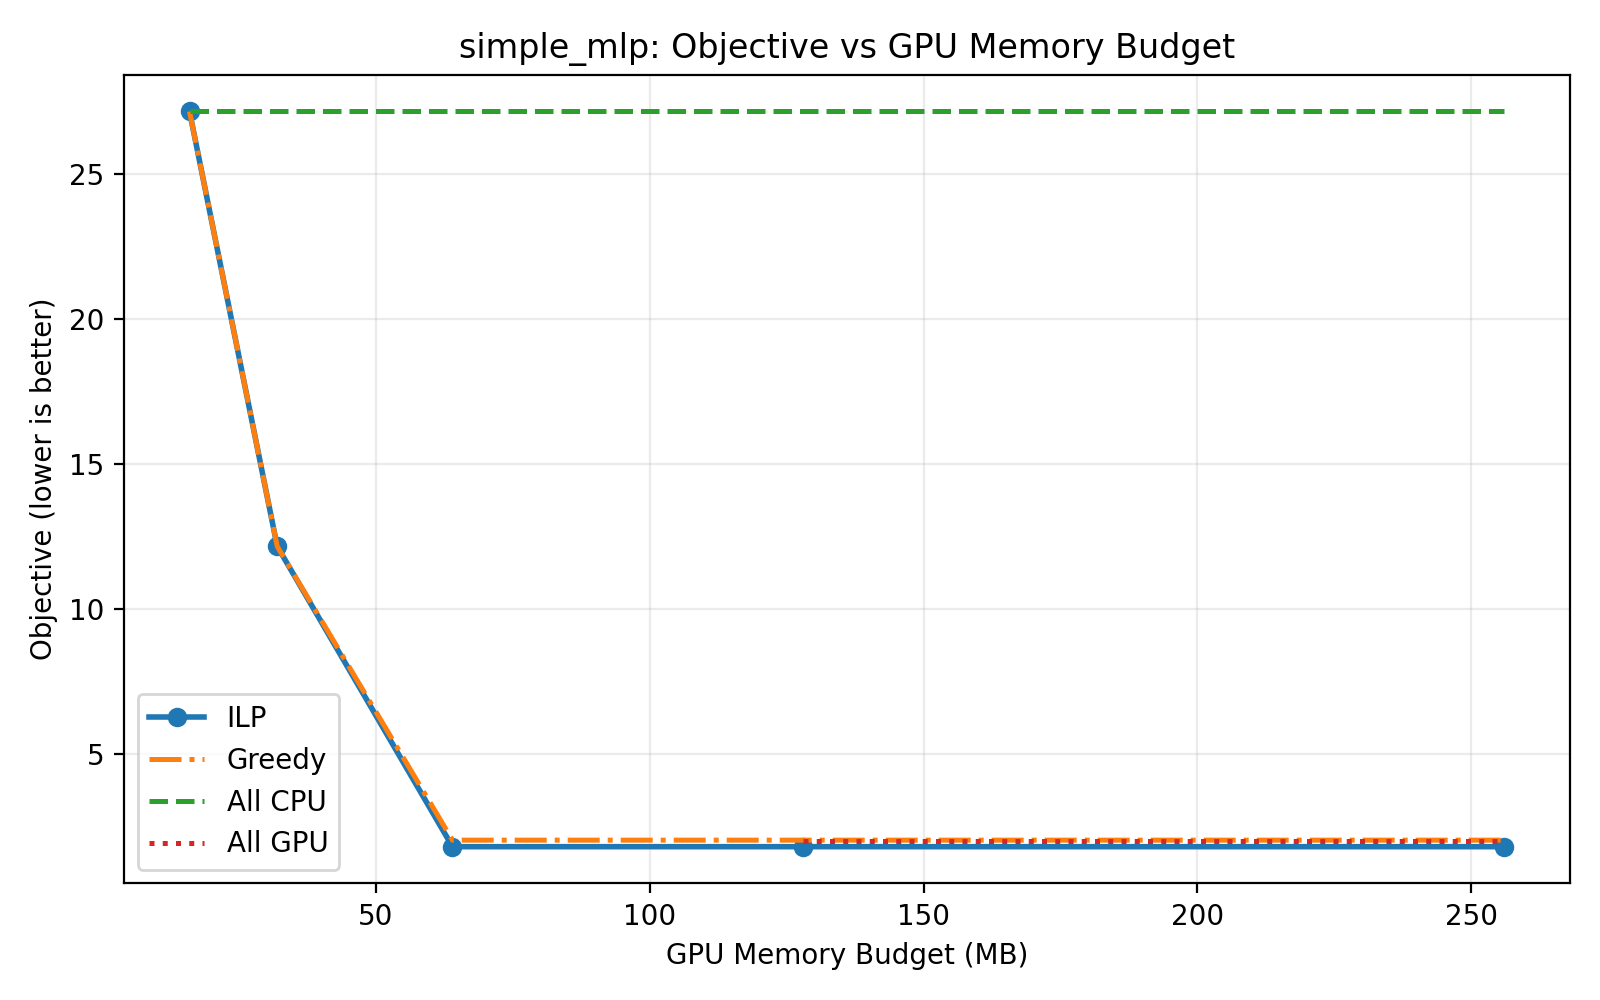
\includegraphics[width=0.78\textwidth]{../reports/ilp_results_phase1_smoke/simple_mlp_objective_vs_budget.png}
\caption{Frontera de compromiso objetivo-presupuesto GPU para el caso smoke consolidado de \code{simple_mlp}.}
\label{fig:ilp-budget-smoke}
\end{figure}

\begin{table}[t]
\centering
\caption{Mejor resultado ILP factible por modelo bajo los presupuestos GPU evaluados en el conjunto smoke.}
\label{tab:ilp-best-per-model-sanitized}
\scriptsize
\resizebox{\textwidth}{!}{%
\begin{tabular}{lrrrrrrrr}
\toprule
Modelo & Budget GPU & Obj. ILP & Obj. CPU & Obj. Greedy & Mejora vs CPU (\%) & Mejora vs Greedy (\%) & Capas GPU & Cortes \\
\midrule
\code{simple_mlp} & 64 & 1.810 & 27.153 & 2.035 & 93.33 & 11.06 & 3 & 1 \\
\bottomrule
\end{tabular}
}
\normalsize
\end{table}

\section{5.11 Estudios de sensibilidad (habilitados por Fase 1)}
Los estudios de sensibilidad muestran que la formulacion no solo produce una solucion puntual, sino una respuesta interpretable ante perturbaciones controladas de sus parametros. En el conjunto smoke, el barrido sobre $k_\sigma$ exhibe una variacion aproximadamente lineal del objetivo en torno al punto base, mientras que el barrido sobre $w_{transfer}$ revela un comportamiento monotono pero no lineal: cuando $w_{transfer}=0.0$, el modelo tolera tres cortes y reordena capas hacia una solucion mas agresiva; al aumentar el peso de transferencia, la politica reduce fragmentacion y encarece el objetivo total bajo una lectura mas conservadora del sistema.

Esta informacion es de interes doctoral porque permite afirmar que los parametros del modelo tienen semantica economica verificable. No son perillas arbitrarias, sino mecanismos de politica cuyo efecto sobre la solucion puede estudiarse con trazas reproducibles.

\section{5.12 Ablaciones formales (habilitadas por Fase 1)}
La suite de ablaciones cumple la funcion de desagregar el aporte de los componentes metodologicos del modelo. En el resumen disponible para \code{simple_mlp}, la variante completa obtiene objetivo 1.810442; eliminar la robustificacion reduce el objetivo en 0.499805 unidades, reflejando un escenario optimista irreal; eliminar topologia o costos de transferencia reduce el objetivo en 0.438429 unidades y altera la estructura de la particion, pasando de un plan con un corte y tres capas en GPU a variantes mas fragmentadas o semantica empobrecida.

Estas ablaciones son importantes porque muestran que la mejora no proviene solo de un solver aplicado sobre cualquier costo disponible. Proviene de la conjuncion entre grafo admisible, penalizacion comunicativa y robustificacion estadistica. En ausencia de alguno de esos componentes, el problema resuelto cambia de significado.

\begin{table}[t]
\centering
\caption{Barrido Pareto ILP en el conjunto smoke con comparacion frente a baselines.}
\label{tab:ilp-budget-sweep-sanitized}
\scriptsize
\resizebox{0.92\textwidth}{!}{%
\begin{tabular}{rrrrrrr}
\toprule
Budget GPU & Obj. ILP & Obj. Greedy & Obj. CPU & Mejora vs CPU (\%) & Mejora vs Greedy (\%) & Cortes \\
\midrule
16 & 27.153 & 27.153 & 27.153 & 0.00 & 0.00 & 0 \\
32 & 12.163 & 12.163 & 27.153 & 55.20 & 0.00 & 1 \\
64 & 1.810 & 2.035 & 27.153 & 93.33 & 11.06 & 1 \\
128 & 1.810 & 2.035 & 27.153 & 93.33 & 11.06 & 1 \\
256 & 1.810 & 2.035 & 27.153 & 93.33 & 11.06 & 1 \\
\bottomrule
\end{tabular}
}
\normalsize
\end{table}

\section{5.13 Extension avanzada: persistencia de activaciones y rematerializacion (Fase 4)}
La extension avanzada deja de ser prospectiva en el estado actual del proyecto. La Fase 4 ha integrado decision dual forward/backward, persistencia de activaciones, recomputacion, checkpointing y compatibilidad con prefetching en \code{src/ilp/advanced_terms.py}, \code{src/ilp/model_builder.py} y en el runtime asociado. Esto permite afirmar que la tesis no se cierra sobre un ILP minimamente viable, sino sobre una version extendida cuyo significado operacional ya fue contrastado en evidencia controlada. La articulacion entre persistencia, recomputacion y particion heterogenea enlaza directamente con la tradicion inaugurada por Revolve y retomada despues por estrategias de memoria sublineal y offloading, aunque aqui se reinterpreta como decision conjunta dentro de una formulacion declarativa unificada \cite{griewank2000revolve,chen2016sublinear,ren2021zerooffload}.

No obstante, desde el punto de vista de escritura doctoral conviene mantener una distincion clara entre dos niveles de evidencia. Existe ya evidencia operacional de que la extension funciona y puede ejecutarse sobre un caso dual controlado; lo que aun falta es una explotacion experimental amplia de esa extension sobre una matriz final de modelos y hosts. El manuscrito debe sostener ambas verdades sin confundir madurez de implementacion con amplitud de validacion empirica.

\section{5.14 Amenazas a la validez}
Las amenazas a la validez del modelo ILP se agrupan en tres clases. La primera es la amenaza de medicion: coeficientes sesgados por ruido, precision degradada o muestra insuficiente pueden inducir optimizaciones sobre un problema mal especificado. La segunda es la amenaza de modelado: la linealidad no captura todas las interacciones no lineales del hardware, como saturacion de bus o contencion compartida. La tercera es la amenaza de transferibilidad: una politica afinada sobre un host unico puede no generalizar a un parque heterogeneo.

Las mitigaciones ya integradas en el proyecto son sustantivas: compuertas de admisibilidad sobre calidad muestral y procedencia estructural, barridos de sensibilidad, ablaciones, comparacion con baselines y capacidad de fusion multi-hardware. Aun asi, el cierre doctoral pleno exige ejecutar el protocolo multi-servidor y ampliar la base de evidencia sobre calidad final del entrenamiento. La necesidad de este cierre adicional no contradice la validez del modelo; la situa, con honestidad, en el mismo horizonte comparativo en el que la literatura reciente ha tenido que conciliar capacidad de optimizacion con diversidad real de plataformas \cite{rajbhandari2020zero,ren2021zerooffload,zheng2022alpa}.

Visto desde una perspectiva mas amplia, este capitulo cumple una funcion que trasciende la simple obtencion de una solucion optima. Su papel es mostrar que la asignacion heterogenea puede formularse como decision cientificamente discutible, y no solo como una heuristica afortunada. El ILP obliga a explicitar hipotesis de costo, restricciones fisicas y relaciones entre nodos y cortes. Esa explicitud es una ganancia epistemologica en si misma, porque permite que el lector cuestione y refine el modelo sin perder de vista que toda modificacion tiene consecuencias operacionales precisas.

\begin{table}[t]
\centering
\caption{Amenazas a la validez del modelo ILP y estado de mitigacion.}
\label{tab:ilp-validity-threats}
\scriptsize
\setlength{\tabcolsep}{4pt}
\begin{tabularx}{\textwidth}{lXX}
\toprule
Amenaza & Mitigacion ya integrada & Evidencia pendiente de cierre \\
\midrule
Medicion sesgada o inestable & Profiling con replicas, robustificacion estadistica, control de precision efectiva y banderas de calidad & Campana multiservidor con base estadistica ampliada \\
Modelo lineal insuficiente & Sensibilidad, ablaciones y contraste posterior con simulacion y runtime & Calibraciones no lineales y estudios de saturacion a mayor escala \\
Falta de transferibilidad entre hosts & Diseno metodologico para fusion multi-hardware y protocolo de validacion transversal & Consolidacion empirica del dataset inter-host y su explotacion final \\
Brecha entre solver y ejecucion real & Representacion formal de plan, simulador y runtime con trazabilidad de procedencia & Matriz mas amplia de contraste prediccion-observacion \\
\bottomrule
\end{tabularx}
\normalsize
\end{table}

La Tabla~\ref{tab:ilp-validity-threats} deja ver que las amenazas a la validez no son un apartado defensivo secundario, sino una parte constitutiva del sentido doctoral del capitulo. Explicitar que esta mitigado, que permanece abierto y bajo que protocolo se resolvera es una forma de honestidad cientifica, pero tambien una forma de fortalecer la interpretabilidad de la solucion obtenida.
